\documentclass[executivepaper]{article}

\usepackage{mathtools}

\everymath{\displaystyle}

\usepackage{amssymb}

\usepackage{commath}

\usepackage{kantlipsum,graphicx}

\usepackage{amsmath}

\usepackage{pgfplots}

\usepackage[utf8]{inputenc}

\usepackage{sectsty}

\usepackage{float}

\sectionfont{\large}

\subsectionfont{\normalsize}

\begin{document}

\renewcommand\thesubsection{\thesection.\arabic{subsection}}

\renewcommand{\ttdefault}{cmtt}

\newtheorem{observation}{Observation}

\vspace*{-25mm}

\begin{center}
	
{\LARGE \textbf{Singular Sturm-Liouville Eigenvalue Problems: Theory and Computation}}

\vspace{3mm}

Brendan D. Busey$^1$ and Stephen B. Robinson$^2$\\ 

\vspace{2mm}

$^1$ Department of Mathematics and Statistics, Wake Forest University\\
Winston-Salem, NC 27109, USA\\

\vspace{2mm}

$^2$ Department of Mathematics and Statistics, Wake Forest University\\
Winston-Salem, NC 27109, USA

\end{center}
	
\vspace{5mm}

\begin{center}

\section*{Abstract}

The focus of the research presented in this paper was, for the singular boundary value problem given as 

\begin{center}

\vspace{-2mm}

\begin{equation}
\begin{array}{l}
\displaystyle (-x^ny')'=\lambda x^my\\[2ex]
\displaystyle y(0)=0, y(1)=0 \\
\end{array} 
\label{eq:BVP}
\end{equation}

\end{center}

defined on the interval $(0,1)$, to examine the affects of changing the value of $m$ and $n$ on the eigenvalues and eigenfunctions that were obtained. The researcher employed the shooting method by numerically solving the initial value problem $(-x^ny')'=\lambda x^my$, defined on the interval $(0,1)$, and subject to the initial conditions $y'(1)=-1, y(1)=0$ for various values of $\lambda$.

\vspace{5mm}

\section*{Introduction}

\end{center}

To begin, we study the eigenvalue-problem

\begin{equation}
\begin{array}{l}
\displaystyle (-x^ny')'=\lambda x^my {~} in {~} (0,1)\\[2ex]
\displaystyle y(0)=0, y(1)=0 \\
\end{array} 
\label{eq:IVP}
\end{equation}

in order to determine the $\lambda$ values such that \eqref{eq:IVP} has a non-trivial solution. We are also interested in exploring how the parameters $n$ and $m$ influence those eigenvalues. Our methods are both experimental and theoretical, with the former relying on the shooting method, while the latter employs solving Euler equations and the method of Frobenius. Through these methods, we hope to characterize the effects of changing the value $n$ and $m$ on the eigenvalues and eigenfunctions. 

\vspace{3mm}

Our research is motivated by the work of Paul Binding and Hans Volkmer who, in $[1]$, discussed the following problem

\vspace{3mm}

\begin{center}

$-(p(x)y')'+q(x)y=(\lambda r(x)+\mu)y,$ for $a \leq x \leq b$.

\end{center}

\pagebreak

\vspace*{-40mm}

with separated boundary conditions $\cos(\alpha)y(a)-\sin(\alpha)p(a)y'(a)=0$ and $\cos(\beta)y(b)-\sin(\beta)p(b)y'(b)=0$.

\vspace{3mm}

\begin{center}

\section*{Research Methodology}

\end{center}

Before proceeding to the main results, to familiarize the reader with the method of research utilized, an overview of the shooting method will be discussed. To begin, we employed the mathematical software Maple in order to plot solutions of the Initial Value Problem \eqref{eq:IVP} for varying values of $m$, $n$, and $\lambda$. Then, in order to document the affects of changing the values of $m$, $n$, and $\lambda$ on the eigenvalues and eigenfunctions, tables were made in order to record the different values for $m$, $n$, $\lambda$, and what behaviour occurred on the $x-axis$ as a result of varying $m$, $n$, and $\lambda$.

\vspace{3mm}

{\centering 

\section*{Experimental Results} \par

}

\subsection*{First Experimental Results: No Eigenvalues}

Below are some of the experimental results that lead to the observation that is presented in the next section.

\begin{center}

\begin{tabular}{||c c c c c c||}

\hline

$\lambda$ & $m$ & $n$ & Roots & $\lim_{x \to 1} y$ & Number of nodes in oscillation \\ [0.5ex]

\hline\hline

4 & 0 & 2 & 0.2 & 0.2 & 1  \\ 

\hline

7 & 0 & 2 & 0.3, 0.1 & 0.1 & 2  \\

\hline

15 & 0 & 2 & 0.45, 0.2, 0.1 & 0.1 & 3  \\

\hline

17 & 0 & 2 & 0.47, 0.22, 0.1 & 0.05 & 4  \\
\hline

22 & 0 & 2 & 0.5, 0.27, 0.12, 0.05 & 0.03 & 5 \\ [1ex]

\hline

\end{tabular}

\vspace{5mm}

Below are graphical representations of the data presented in the above table

\begin{figure}[H]

\centering

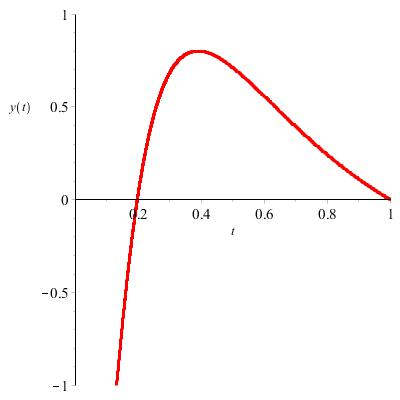
\includegraphics[width=0.5\textwidth]{NEquals2MEquals0LambdaEquals4}

\caption{$n=2$, $m=0$, and $\lambda=4$}

\end{figure}

\pagebreak

\vspace*{-40mm}

\begin{figure}[H]

\centering

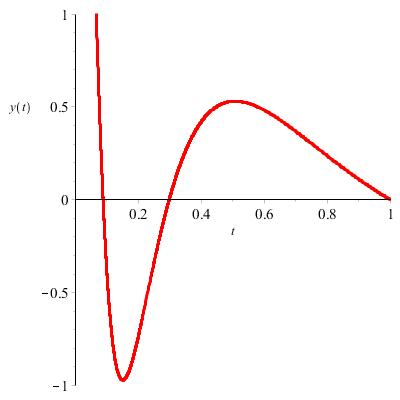
\includegraphics[width=0.5\textwidth]{NEquals2MEquals0LambdaEquals7}

\caption{$n=2$, $m=0$, and $\lambda=7$}

\end{figure}

\begin{figure}[H]

\centering

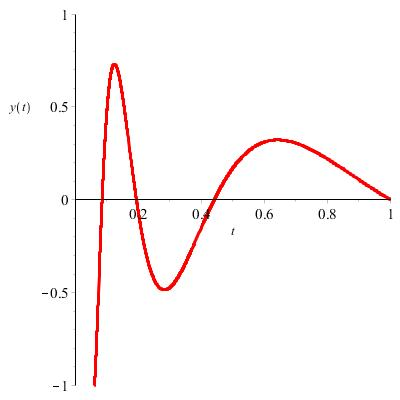
\includegraphics[width=0.5\textwidth]{NEquals2MEquals0LambdaEquals15}

\caption{$n=2$, $m=0$, and $\lambda=15$}

\end{figure}

\pagebreak

\vspace*{-40mm}

\begin{figure}[H]

\centering

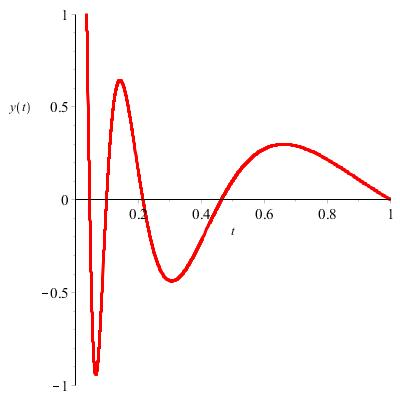
\includegraphics[width=0.5\textwidth]{NEquals2MEquals0LambdaEquals17}

\caption{$n=2$, $m=0$, and $\lambda=17$}

\end{figure}

\vspace{5mm}

\begin{figure}[H]

\centering

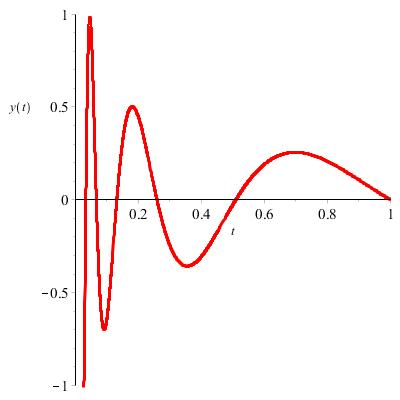
\includegraphics[width=0.5\textwidth]{NEquals2MEquals0LambdaEquals22}

\caption{$n=2$, $m=0$, and $\lambda=22$}

\end{figure}

\end{center}

\pagebreak

\vspace*{-40mm}

\subsection*{First Theoretical Result: Euler equation solutions}

We first considered solutions that were in the form of \textit{Euler equations}. An Euler equation, as defined in [2], is a relatively simple differential equation that has a singular point, or a point at which the Euler equation cannot be represented by a power series of the form $\sum_{n=0}^{\infty} a_{n} x^n$. As such, we say that an Euler equation is analytic. Euler equations are of the form

\begin{center}

$x^2y''+\alpha xy'+\beta y=0$, where $\alpha$ and $\beta$ are real constants.

\end{center}

\subsection*{Method Summary}

In the first experimental results section, we observed how \eqref{eq:IVP} displayed asymptotic behaviour as it approached the origin based on the the values for $\lambda$. We will now verify this observation for well-chosen values for $m$ and $n$.

\begin{observation}

With our well-chosen, positive $n$ values, asymptotic behaviour, specifically a vertical asymptote, occurs along the $x-axis$, regardless of the value of $m$
 
\end{observation}

\vspace{3mm}

Recall, that the problem we are studying is of the form

\begin{center}

$(-x^ny')'=\lambda x^my$, subject to the boundary conditions $y(0)=0, y(1)=0$.

\end{center}

Then, if we subtract the $\lambda x^my$ term from both sides we have:

\begin{center}

$(-x^ny')'-\lambda x^my=0$

\end{center}

Now, taking the first derivative, we have:

\begin{center}

$-x^ny''-nx^{n-1}y'-\lambda x^my=0$

\end{center}

\vspace{3mm}

Now, suppose the solutions are of the form $y=x^r$. Then, $y'=rx^{r-1}$ and $y''=r(r-1)x^{r-2}$. Plugging the derivatives we just took back into the original differential equation, we have:

\begin{center}

$-x^2(r(r-1)x^{r-2})-nx^1(rx^{r-1})-\lambda(x^r)=0$

\hspace{1mm}

$-x^2(x^{-2} \cdot x^r \cdot r(r-1))-nx^1(x^{-1} \cdot x^r \cdot r)-\lambda \cdot x^r=0$

\hspace{1mm}

$(-x^r \cdot r(r-1))-n(x^r \cdot r)-\lambda \cdot x^r=0$

\vspace{3mm}

Factoring out a common factor of $x^r$ and then multiplying through by $-1$, we have:

\vspace{3mm}

$x^r \bigg[(r(r-1)+nr+\lambda \bigg]=0$

\hspace{1mm}

$r(r-1)+nr+\lambda=0$, which is our characteristic equation

\end{center}

Now, in order to find the roots of our characteristic equation, we use the quadratic formula:

\pagebreak

\vspace*{-40mm}

\begin{center}

$\frac{-(n-1) \pm \sqrt{(n-1)^2-4(\lambda)}}{2(1)}$

\hspace{1mm}

$\implies \frac{-n+1 \pm \sqrt{(n-1)^2-4 \lambda}}{2}$

\hspace{1mm}

$\implies \frac{1-n \pm \sqrt{(n-1)^2-4 \lambda}}{2}$

\vspace{3mm}

Now, using $n=2$, we now have:

\vspace{2mm}

$\implies \frac{1-2 \pm \sqrt{(2-1)^2-4 \lambda}}{2}$

\hspace{1mm}

$\implies \frac{-1 \pm \sqrt{1-4 \lambda}}{2}$

\hspace{1mm}

$\implies \frac{-1}{2} \pm \sqrt{\frac{1}{4}-\lambda}$

\end{center}

Now, if we recall that we supposed that our solutions were of the form $y=x^r$ and denote our two solutions as $y_{1}$ and $y_{2}$, we have: 

\begin{center}

$y_{1}(x)=x^{r_{1}}=x^{-\frac{1}{2}+\sqrt{\frac{1}{4}-\lambda}}=x^{-\frac{1}{2}}x^{\sqrt{\frac{1}{4}-\lambda}}$

\hspace{1mm}

$y_{2}(x)=x^{r_{2}}=x^{-\frac{1}{2}-\sqrt{\frac{1}{4}-\lambda}}=x^{-\frac{1}{2}}x^{-\sqrt{\frac{1}{4}-\lambda}}$

\end{center}

So, the equation for our general solution will take the form:

\begin{center}

$y(x)=c_{1}x^{r_{1}}+c_{2}x^{r_{2}}$

\end{center}

Substituting back in for $x^{r_{1}}$ and $x^{r_{2}}$, we have:

\begin{center}

$y(x)=c_{1}x^{-\frac{1}{2}}x^{\sqrt{\frac{1}{4}-\lambda}}+c_{2}x^{-\frac{1}{2}}x^{-\sqrt{\frac{1}{4}-\lambda}}$

\end{center}

Next, if we use the initial condition $y(0)=1$, we get:

\begin{center}

$y(0)=c_{1}(1)^{-\frac{1}{2}}(1)^{\sqrt{\frac{1}{4}-\lambda}}+c_{2}(1)^{-\frac{1}{2}}(1)^{-\sqrt{\frac{1}{4}-\lambda}}$

\hspace{1mm}

$y(x)=c_{1}+c_{2}$

\end{center}

Now, consider specifically, $\sqrt{\frac{1}{4}-\lambda}$ \vspace{1mm} :

\begin{center}

$\sqrt{\frac{1}{4}-\lambda}=\sqrt{(-1)\bigg(\lambda - \frac{1}{4}\bigg)}=i\sqrt{\bigg(\lambda - \frac{1}{4}\bigg)}$

\end{center}

In this case, we want to only consider the real roots, so we have to extract them using Euler's formula:

\begin{center}

let $x^{\alpha i}=(e^{\ln(x)})^{\alpha i}=e^{\alpha \ln(x) i}$

\hspace{1mm}

using $e^{\alpha \ln(x) i}$ and $\alpha=\sqrt{\lambda-\frac{1}{4}}$, we have:

\hspace{1mm}

$\cos(\alpha \ln(x))+i\sin(\alpha \ln(x))=\cos\bigg(\sqrt{\lambda-\frac{1}{4}} \ln(x)\bigg)+i\sin\bigg(\sqrt{\lambda-\frac{1}{4}} \ln(x)\bigg)$

\end{center}

\pagebreak

\vspace*{-40mm}

Now, earlier, we had shown our two solutions were:

\begin{center}

$y_{1}(x)=x^{-\frac{1}{2}}x^{\sqrt{\frac{1}{4}-\lambda}}$

\hspace{1mm}

$y_{2}(x)=x^{-\frac{1}{2}}x^{-\sqrt{\frac{1}{4}-\lambda}}$

\end{center}

However, if we now update our solutions using the results from Euler's formula, we have:

\begin{center}

$y_{1}(x)=x^{-\frac{1}{2}}\cos\bigg(\sqrt{\lambda-\frac{1}{4}} \ln(x)\bigg)$

\hspace{1mm}

$y_{2}(x)=x^{-\frac{1}{2}}sin\bigg(\sqrt{\lambda-\frac{1}{4}} \ln(x)\bigg)$

\end{center}

Finally, the astute reader can conclude that the components of the supposed solution will oscillate and become infinitely large as $x \rightarrow 0$, causing the previously defined asymptotic behaviour, as proposed in $Observation \ 1$

\subsection*{Second Experimental Results: Existence of Eigenvalues}

\begin{tabular}{||c c c c c c||}

\hline

$\lambda$ & $m$ & $n$ & Roots & $\lim_{x \to 1} y$ & Number of nodes in oscillation \\ [0.5ex]

\hline\hline

39 & -1 & 1 & 1,0 & 0 & 1  \\ 

\hline

160 & -1 & 1 & 1, 0.7 & 0 & 2  \\

\hline

355 & -1 & 1 & 1, 0.8, 0.6, 0 & 0 & 3  \\

\hline

640 & -1 & 1 & 1, 0.88, 0.7, 0.5, 0 & 0 & 4  \\
\hline

990 & -1 & 1 & 1, 0.9, 0.78, 0.62, 0.42, 0 & 0 & 5 \\ [1ex]

\hline

\end{tabular}

\vspace{5mm}

Below are the graphical representations of the data presented in the above table

\begin{figure}[H]

\centering

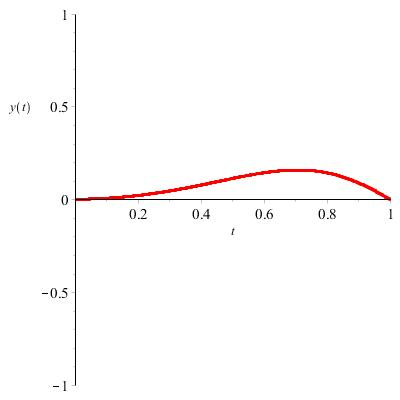
\includegraphics[width=0.5\textwidth]{NEqualsNegative1MEquals1LambdaEquals39}

\caption{$n=-1$, $m=1$, and $\lambda=39$}

\end{figure}

\begin{figure}[H]

\centering

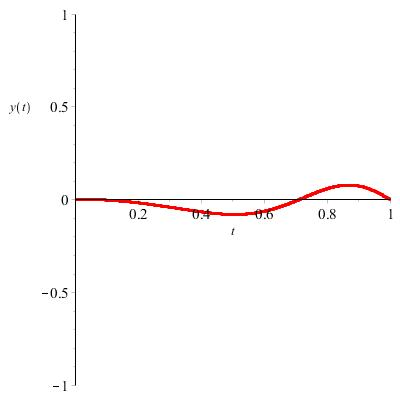
\includegraphics[width=0.5\textwidth]{NEqualsNegative1MEquals1LambdaEquals160}

\caption{$n=-1$, $m=1$, and $\lambda=160$}

\end{figure}

\begin{figure}[H]

\centering

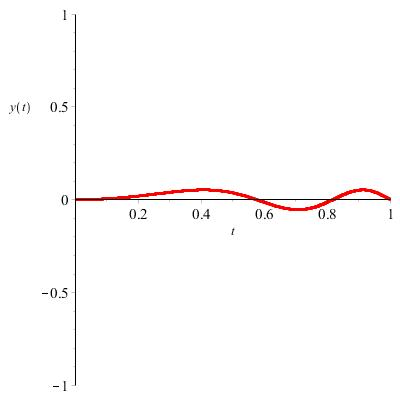
\includegraphics[width=0.5\textwidth]{NEqualsNegative1MEquals1LambdaEquals355}

\caption{$n=-1$, $m=1$, and $\lambda=355$}

\end{figure}

\begin{figure}[H]

\centering

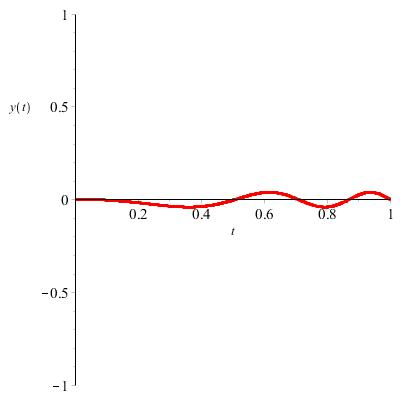
\includegraphics[width=0.5\textwidth]{NEqualsNegative1MEquals1LambdaEquals640}

\caption{$n=-1$, $m=1$, and $\lambda=640$}

\end{figure}

\vspace{5mm}

\begin{figure}[H]

\centering

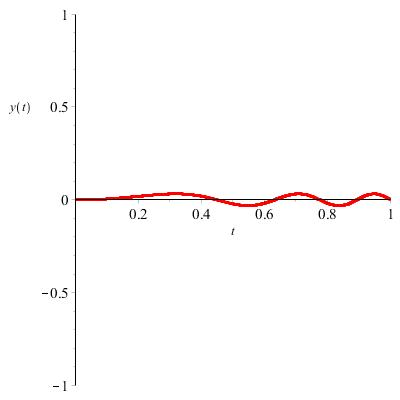
\includegraphics[width=0.5\textwidth]{NEqualsNegative1MEquals1LambdaEquals990}

\caption{$n=-1$, $m=1$, and $\lambda=990$}

\end{figure}

\pagebreak

\vspace*{-40mm}

\subsection*{Second Theoretical Result: Power Series Solutions}

In the first theoretical section, we considered the case where we were able to solve \eqref{eq:IVP} using Euler equations. However, for the following case, we will shift from using Euler equations to employing Power Series in order to find solutions for \eqref{eq:IVP}.

\subsection*{Method Summary}

In the second experimental section, we observed how the roots of \eqref{eq:IVP} became more and more clustered as \eqref{eq:IVP} approached the origin based on the the values for $\lambda$. We will now verify this observation for well-chosen values for $m$ and $n$.

\begin{observation}

When $m$ is greater than $n$, $n$ is negative or zero, and as lambda values increases, the roots become clustered closer together.
 
\end{observation}

\vspace{3mm}

Before we verify this observation for our well-chosen values for $m$ and $n$, recall that in the first theoretical section, we were interested in solutions determined using Euler equations which took the general form of

\begin{center}

$x^2y''+\alpha xy'+\beta y=0$, where $\alpha$ and $\beta$ are real constants.

\end{center}

In this section, however, we consider the general problem of determining a solution of the equation

\begin{center}

$x^2y'' + x[xp(x)]y' + [x^2q(x)]y=0$

\end{center}

for our well-chosen values of $m$ and $n$. With that out of the way, recall that the problem we are considering is

\begin{center}

$(-x^ny')'=\lambda x^my$, subject to the boundary conditions $y(0)=0, y(1)=0$

\end{center}

Then, if we subtract the $\lambda x^my$ term from both sides, we have:

\begin{center}

$(-x^ny')'-\lambda x^my=0$

\end{center}

Now, taking the first derivative, we have:

\begin{center}

$-x^ny''-nx^{n-1}y'-\lambda x^my=0$

\end{center}

If we then divide through by negative one, we obtain:

\begin{center}

$x^ny''+nx^{n-1}y'+\lambda x^my=0$

\end{center}

If we make the substitution for our well-chosen values of $n=-1$ and $m=1$, we have:

\begin{center}

$x^{-1}y''+nx^{-1-1}y'+\lambda x^2y=0$

\vspace{2mm}

$x^{-1}y''+nx^{-2}y'+\lambda x^2y=0$

\end{center}

Next, if we multiply through by $x^3$, we get:

\pagebreak

\vspace*{-40mm}

\begin{center}

$x^2y''-xy'+\lambda x^4y=0$

\end{center}

Now, since we interested in observing the behaviour of \eqref{eq:IVP} on the interval $(0,1)$, we will verify that $x=0$ is a regular singular point. So, in our case

\begin{center}

$xp(x)=-1$ $\quad$ and $\quad$ $x^2q(x)=\lambda x^4$

\end{center}

and if we take the limit as $x \rightarrow 0$, we get

\begin{center}

$\lim_{x \to 0} xp(x)=-1$ $\quad$ and $\quad$ $\lim_{x \to 0} x^2q(x)=0$

\end{center}

Since both limits exist, we have that $x=0$ is a regular singular point. So, by \textit{Theorem 5.6.1} on pages $293$ and $294$ from the chapter on Series Solutions Near a Regular Singular Point from [2], we have that $xp(x)$ and $x^2q(x)$ are analytic at $x=0$, with convergent power series expansions of the following form

\begin{center}

$xp(x)=\sum_{n=0}^{\infty} p_{n} x^{n}$ $\quad$ and $\quad$ $x^2q(x)=\sum_{n=0}^{\infty} q_{n} x^{n}$

\end{center}

Now, the astute reader can easily verify that at $n=0$, 

\begin{center}

$\sum_{n=0}^{\infty} p_{n} x^{n}=-1$ $\quad$ and $\quad$ $\sum_{n=0}^{\infty} q_{n} x^{n}=0$

\end{center}

So, now, let $r_{1}$ and $r_{2}$ be the roots of the indicial equation equation

\begin{center}

$F(r)=r(r-1)+p_{0}r+q_{0}=0$

\end{center}

Then, if we substitute in for our $p_{0}$ and $q_{0}$, our indicial equation becomes

\begin{center}

$F(r)=r(r-1)-r=0$

\end{center}

Solving for $r$, we find

\begin{center}

$r(r-1)-r=0$

\vspace{2mm}

$\implies r^2-r-r=0$

\vspace{2mm}

$\implies r^2-2r=0$

\vspace{2mm}

$\implies r(r-2)=0$

\vspace{2mm}

$\implies r_{1}=2$ $\quad$ and $\quad$ $r_{2}=0$

\end{center}

So, by our previous theorem (5.6.1), we know that our first solution will be of the form

\begin{center}

$y_{1}(x)=\abs{x_{1}}^{r_{1}} \bigg[1 + \sum_{n=1}^{\infty} a_{n}(r_{1})x^n\bigg]$

\end{center}

and, since $r_{1}-r_{2}=2$, a positive integer, we know that our second solution will be of the form

\pagebreak

\vspace*{-40mm}

\begin{center}

$y_{2}(x)=ay_{1}(x) \ln{\abs{x}} + \abs{x}^{r_{2}} \bigg[1 + \sum_{n=1}^{\infty} c_{n}(r_{2})x^n\bigg]$

\end{center}

Then, if we substitute appropriately for $r_{1}$ and $r_{2}$, our solutions become

\begin{center}

$y_{1}(x)=\abs{x_{1}}^{r_{1}} \bigg[1 + \sum_{n=1}^{\infty} a_{n}(r_{1})x^n\bigg]$

\vspace{2mm}

$y_{1}(x)=\abs{x_{1}}^{2} \bigg[1 + \sum_{n=1}^{\infty} 2a_{n}x^n\bigg]$

\end{center}

and

\begin{center}

$y_{2}(x)=ay_{1}(x) \ln{\abs{x}} + \abs{x}^{r_{2}} \bigg[1 + \sum_{n=1}^{\infty} c_{n}(r_{2})x^n\bigg]$

\vspace{2mm}

$y_{2}(x)=ay_{1}(x) \ln{\abs{x}} + \abs{x}^{0} \bigg[1 + \sum_{n=1}^{\infty} c_{n}(0)x^n\bigg]$

\vspace{2mm}

$y_{2}(x)=ay_{1}(x) \ln{\abs{x}} + \bigg[1 + \sum_{n=1}^{\infty} 0 \bigg]$

\vspace{2mm}

$y_{2}(x)=a \abs{x_{1}}^{2} \bigg[1 + \sum_{n=1}^{\infty} 2a_{n}x^n\bigg] \ln{\abs{x}} + 1$

\end{center}

Finally, the astute reader can see that as we take the limit as $x \rightarrow 0$, both solutions, $y_{1}(x)$ and $y_{2}(x)$, we go to zero, as well any linear combination of these two solutions.

\pagebreak

\vspace*{-40mm}

\begin{center}

\begin{thebibliography}{9}

\bibitem{EigencurvesForTwoParameter} 
Binding, Paul; Volkmer, Hans
\textit{Eigencurves for two-parameter Sturm-Liouville equations. SIAM Rev. 38 (1996), no. 1, 27---48}.

\vspace{1mm}

\bibitem{ElementaryDifferentialEquationsAndBoundaryValueProblems}
Boyce, William E.; DiPrima, Richard C.
\textit{Elementary differential equations and boundary value problems. John Wiley \& Sons, Inc., New York-London-Sydney 1965 xi+485 pp. 34.00}. 

\end{thebibliography}

\end{center}

\end{document}